
\section{Architektur}
\label{sec:Architektur}

In diesem Kapitel wird die Architektur unserer Applikation und die Schnittstellen zu den Umsystemen besprochen. Als Anhaltspunkt wird das C4 Modell \cite{c4model} von Simon Brown verwendet. In einem ersten Schritt wird unsere Applikation in den Kontext des grösseren Systems gesetzt. Anschliessend teilen wir das System \emph{PlazaRoute} in einzelne Container und den zentralen Container \emph{Plaza Routing} in einzelne Komponenten auf.

\subsection{Systemkontext}
\label{architektur:Systemkontext}

\begin{figure}[ht]
    \centering
    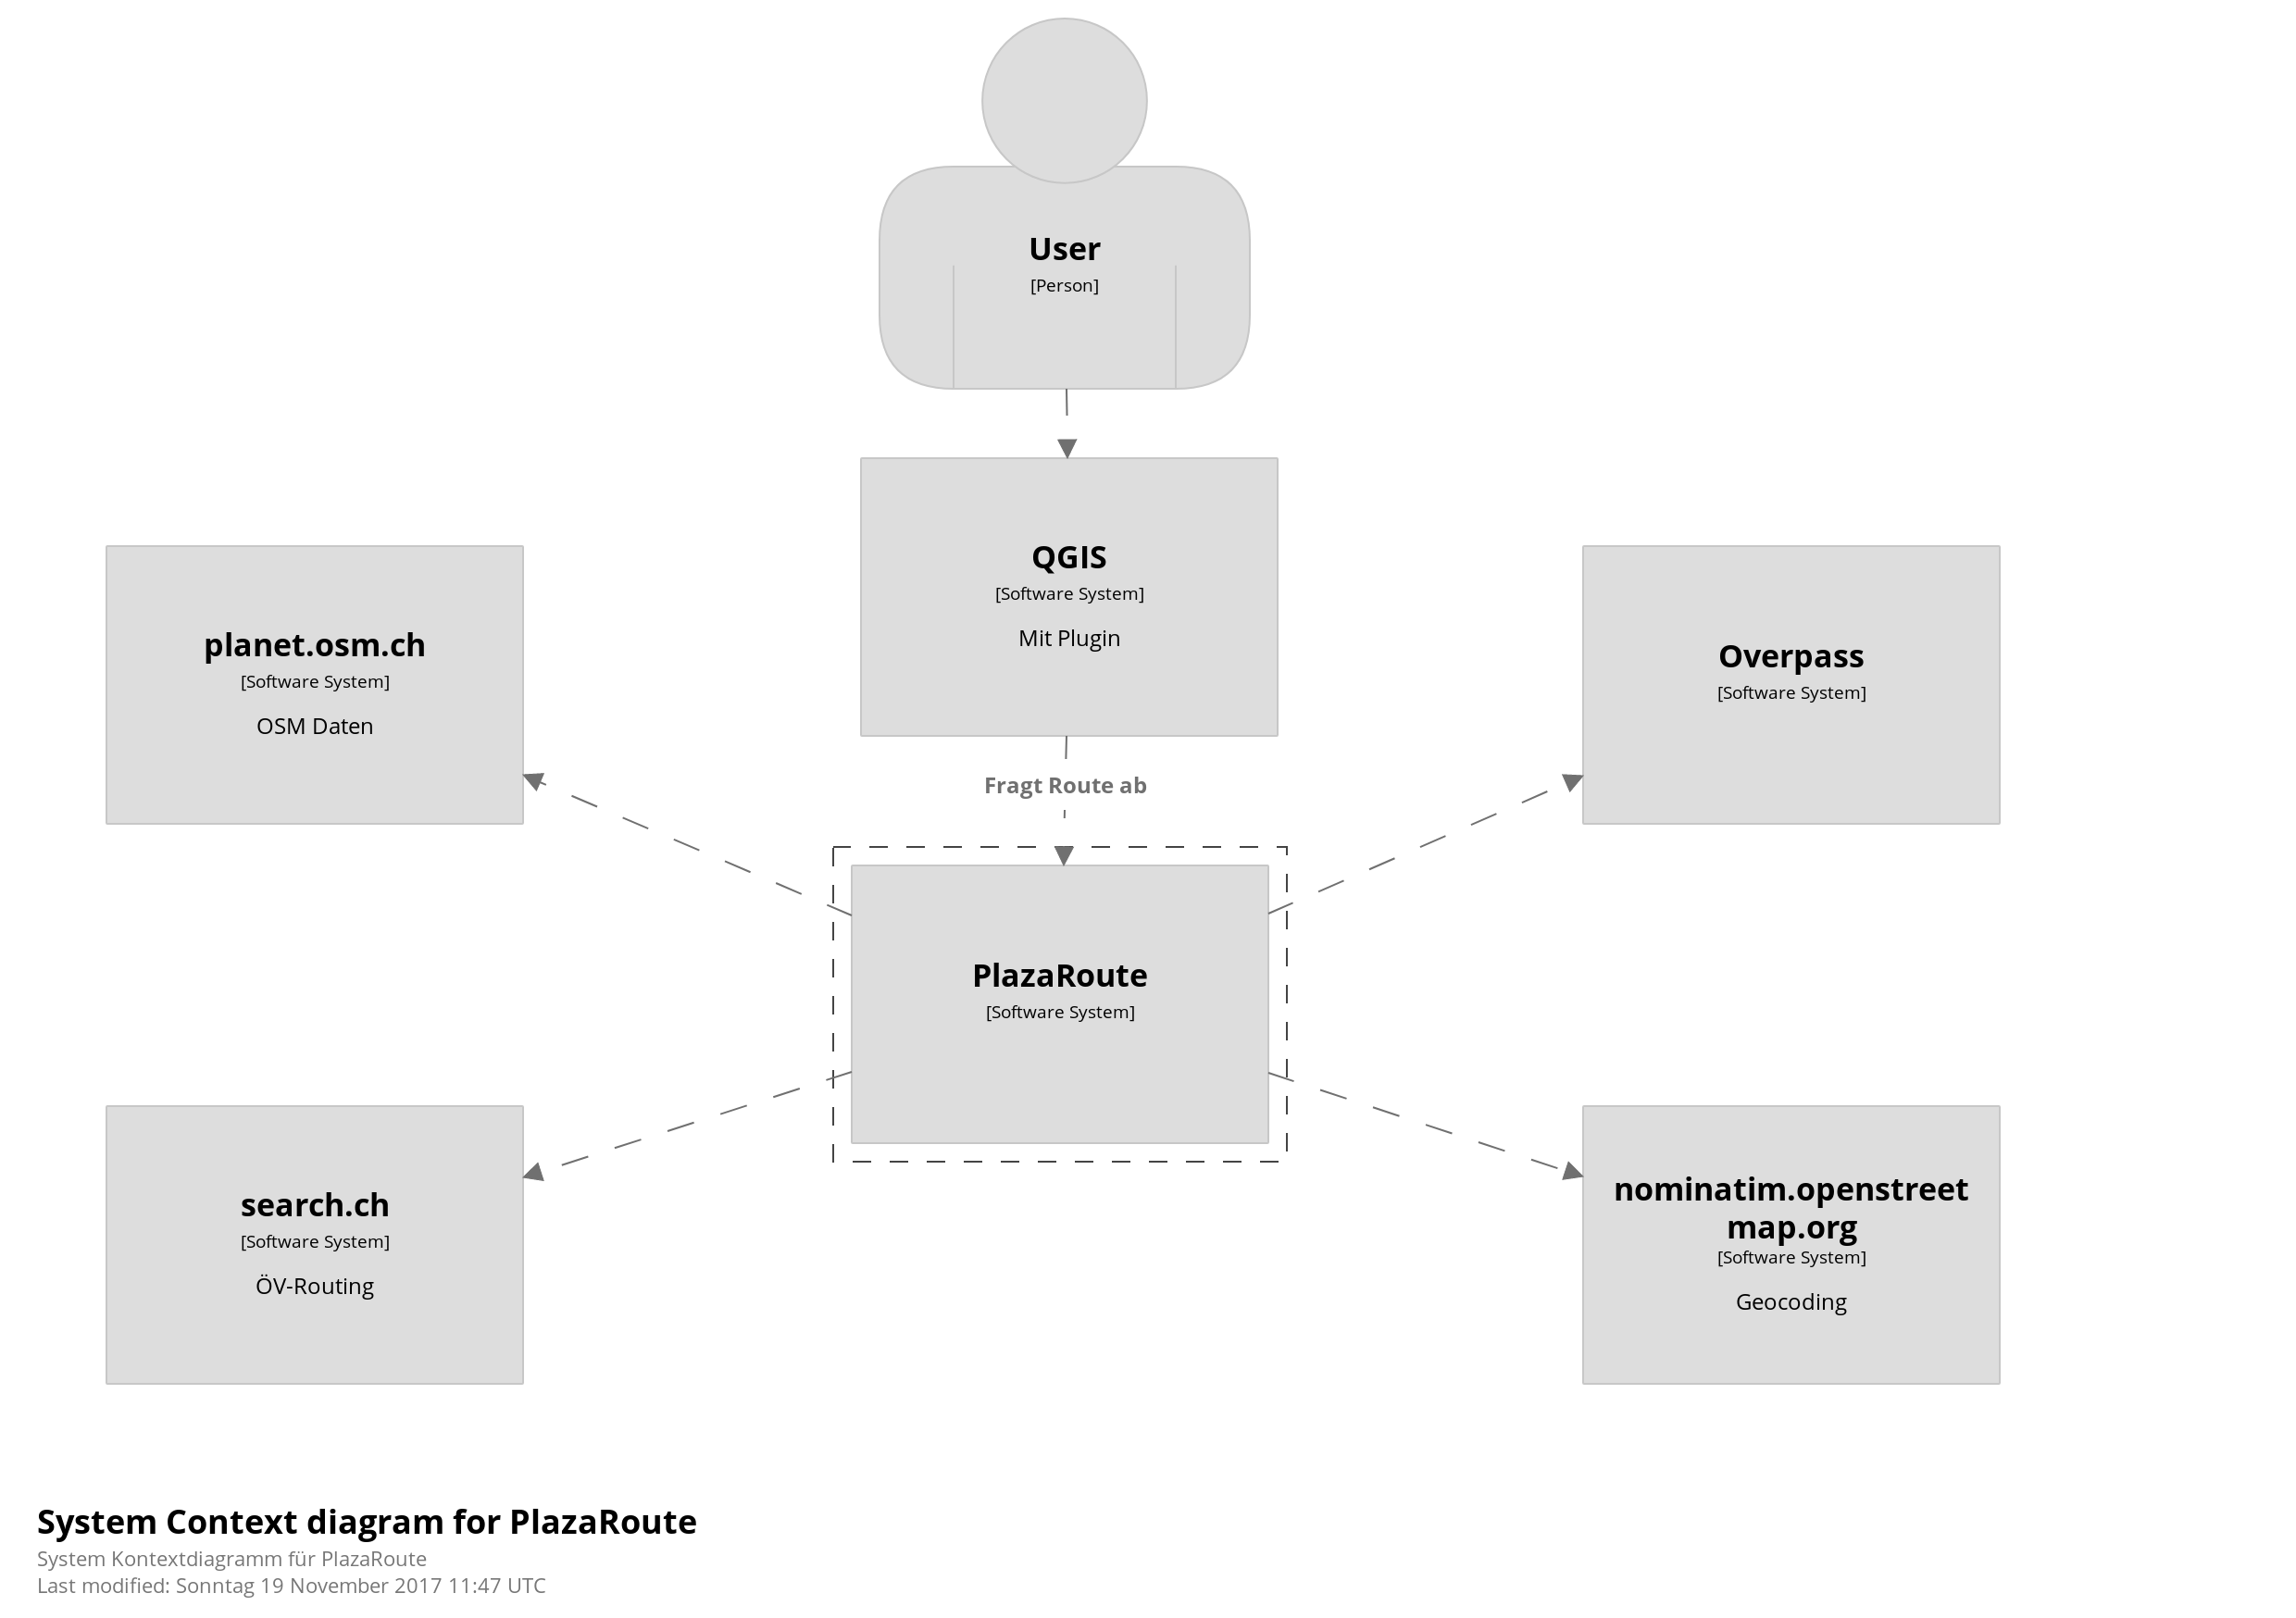
\includegraphics[width=1\linewidth]{projectdoc/img/system-context_diagram.png}
    \caption[System Kontext Diagramm]{System PlazaRoute im Kontext mit Umsystemen; Grafik erstellt mit \emph{Structurizr Express}\cite{structurizr}}
    \label{fig:system_context_diagram}
\end{figure}

Abbildung \ref{fig:system_context_diagram} zeigt das System PlazaRoute mit den Umsystemen auf. Beim Betrachten der C4-Diagramme ist zu beachten, dass diese nicht der \acs{UML}-Spezifikation folgen. Gestrichelte Pfeile bedeuten, dass eine Anfrage in Richtung der Pfeilspitze an ein System geht. Der Datenfluss läuft in die entgegengesetzte Richtung der Pfeile.

Der User bedient die QGIS Desktop Applikation mit dem von uns entwickelten Plugin. Dieses leitet die die Eingabe der Start- und Zielkoordinaten an das System PlazaRoute weiter. Als Antwort sendet PlazaRoute eine Routenbeschreibung an das QGIS-Plugin zurück, das es im QGIS darstellt.

\subsection{PlazaRoute Container}
\label{architektur:PlazaRoute Container}

\begin{figure}[ht]
    \centering
    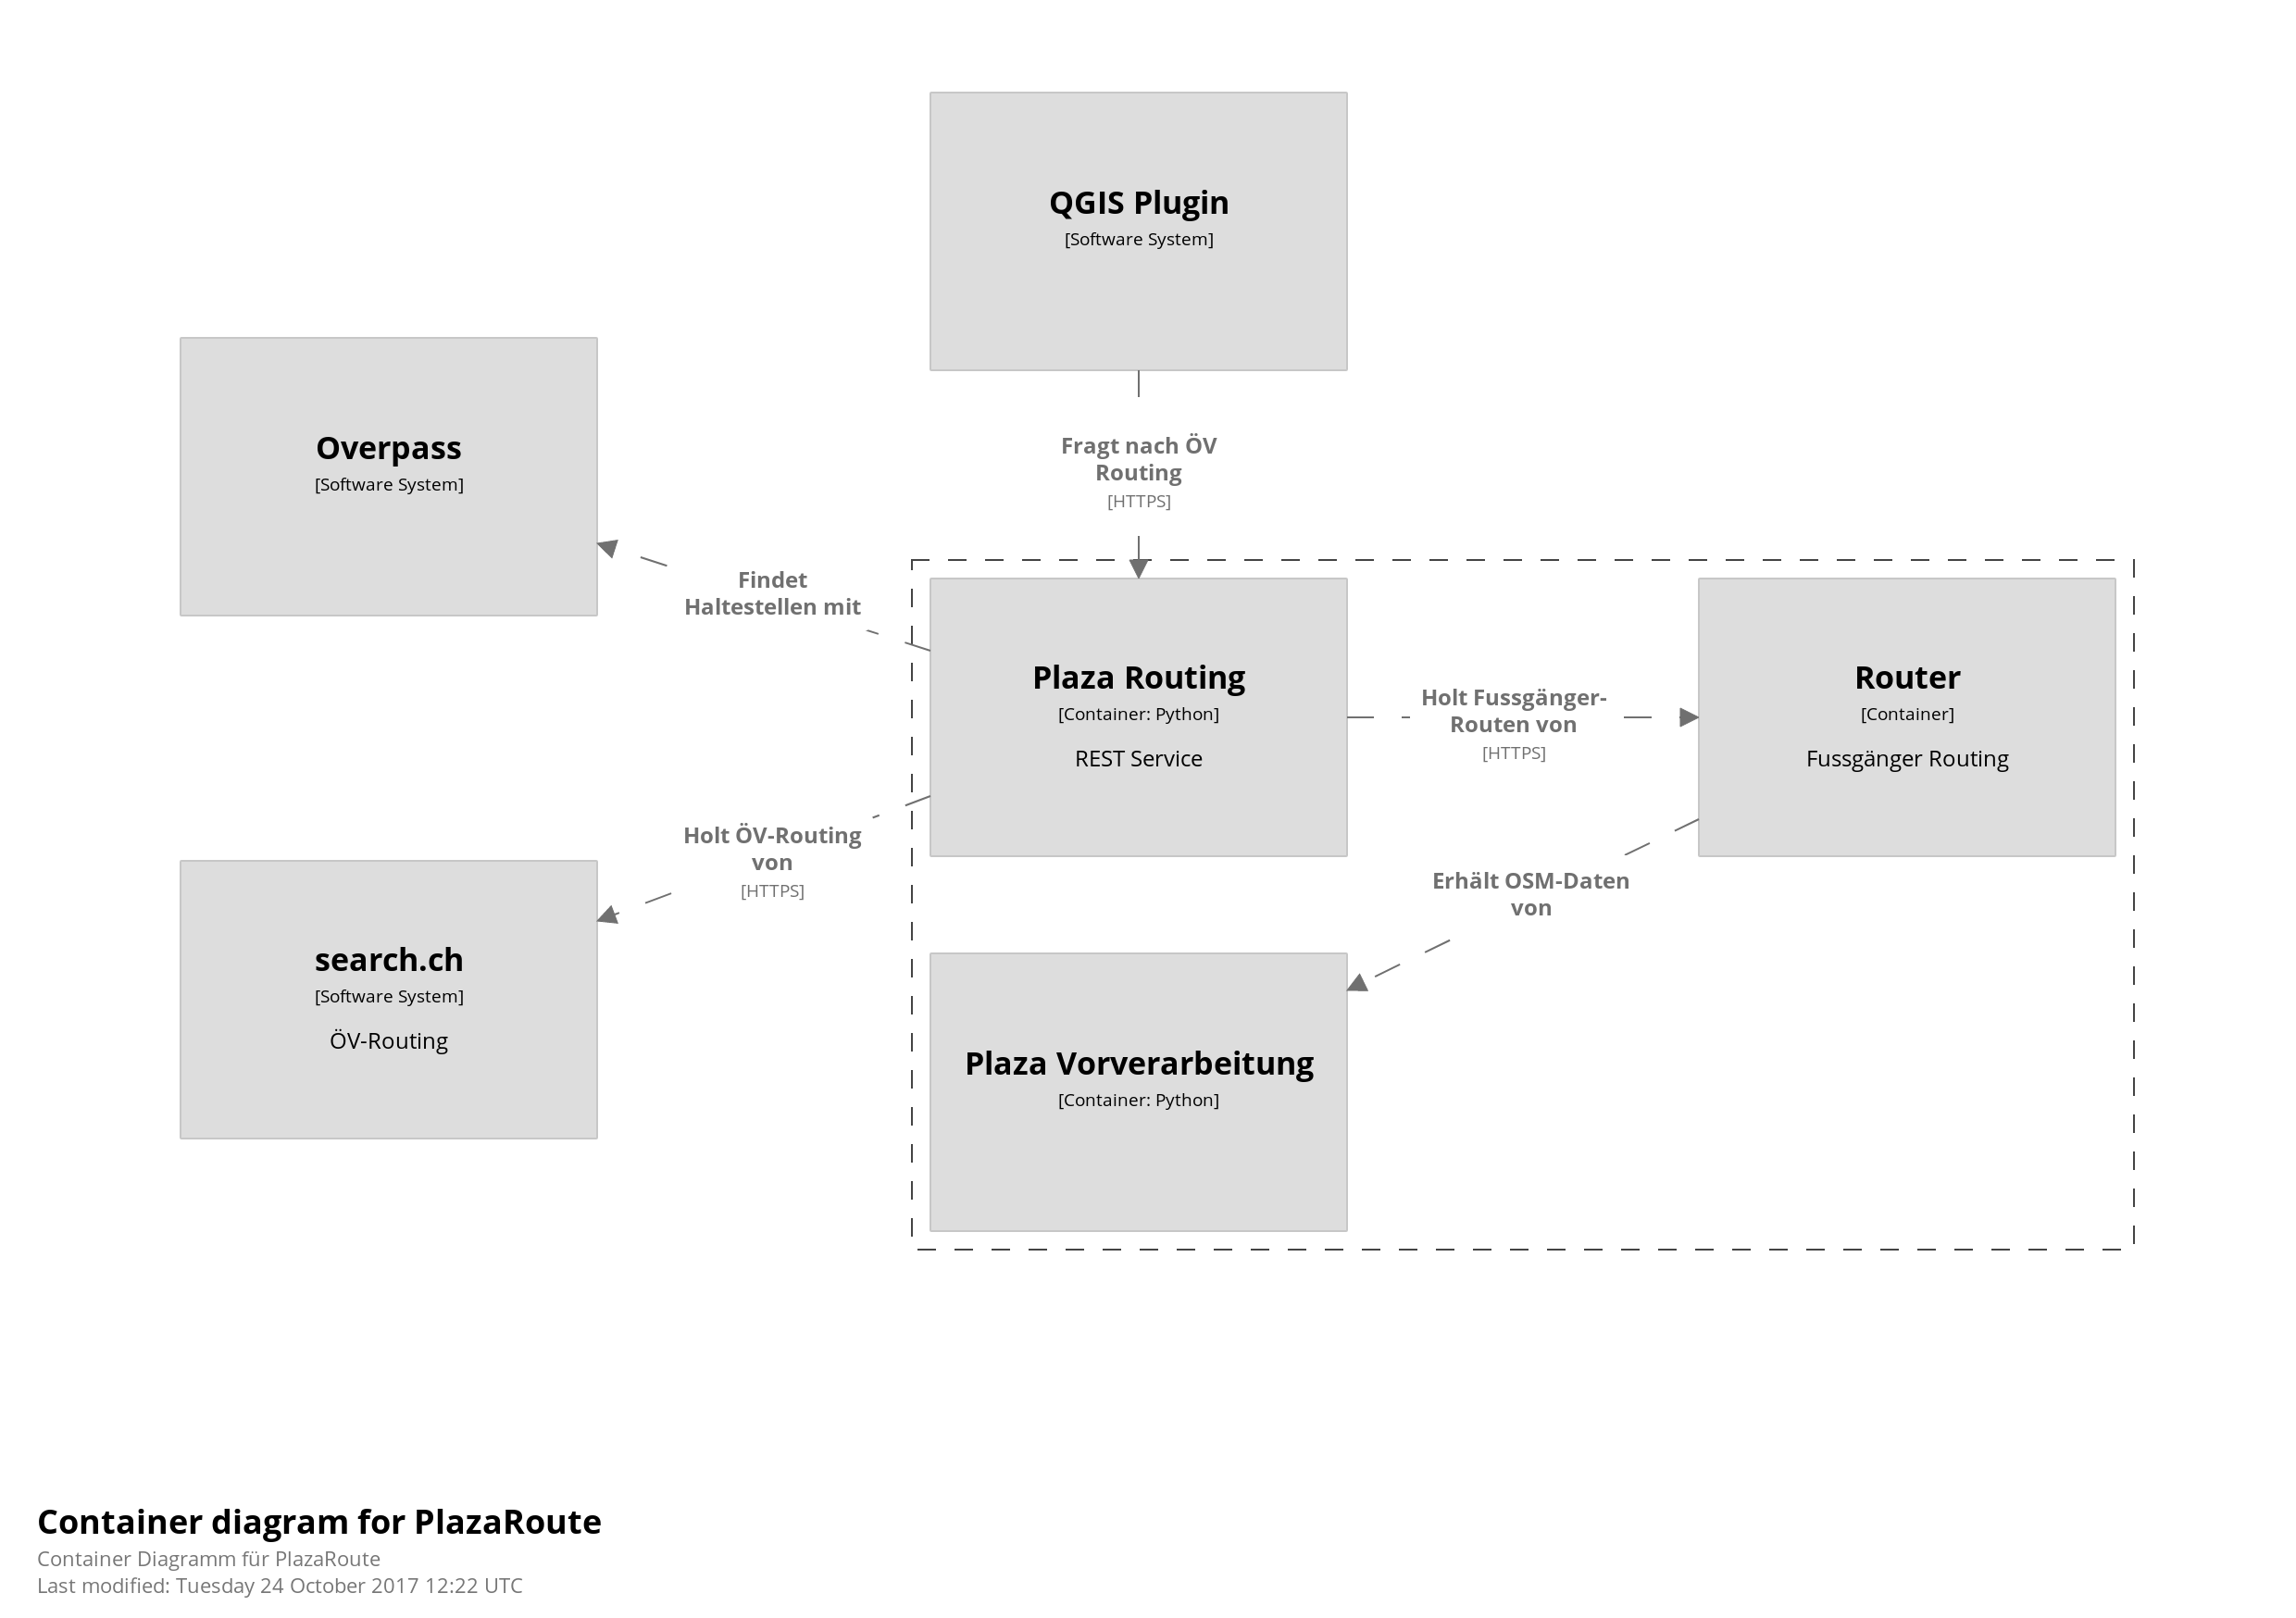
\includegraphics[width=1\linewidth]{projectdoc/img/container_diagram.png}
    \caption[Container Diagramm]{Container Diagramm von PlazaRoute; Das System PlazaRoute befindet sich in der eingerahmten Box; Grafik erstellt mit \emph{Structurizr Express}\cite{structurizr}}
    \label{fig:container_diagram}
\end{figure}

In Abbildung \ref{fig:container_diagram} zoomen wir in das System PlazaRoute hinein und teilen es in drei Container auf, die logisch voneinander getrennt sind. So könnten die Container auch verteilt deployed werden.

In den nachfolgenden Abschnitten werden die drei Container näher beleuchtet.


\subsubsection{Plaza Vorverarbeitung}
\label{architektur:Plaza Vorverarbeitung}

Bevor die Routing Engine ihre Routing-Funktion ausführen kann, muss diese zuerst aus dem \ac{OSM}-Datensatz einen Routing-Graph generieren. Unsere Hauptaufgabe besteht darin, diesen Routing-Graphen für Fussgänger-Routing über Flächen zu optimieren. Ein Ansatz wäre, den Graphen nach dem Generieren zu verändern. Dies ist aber schwer realisierbar, da die meisten Routing-Engines die Graphen in eigenen (binären) Datenstrukturen ablegen. So wär unsere Implementation auch stark an eine einzelne Routing-Engine gekoppelt.

Ein zweiter Ansatz die Integration unserer Optimierung in die Verarbeitung der Routing-Engines selbst. Auch da wären wir wieder stark an eine spezifische Routing-Engine gekoppelt.
Wir haben uns stattdessen entschieden, beim Input der \ac{OSM}-Daten anzusetzen. Dazu werden die Rohdaten zuerst eingelesen und nach Fussgänger-Flächen abgesucht (\nameref{par:OSM Importer}). Mit unserem Algorithmus werden neue Fusswege eingetragen (\nameref{par:Plaza Optimizer}). Diese neu erzeugten Kartendaten werden dann wieder mit den ursprünglichen Rohdaten verschmelzt (\nameref{par:OSM Merger}). Erst dann generiert die Routing-Engine daraus den Routing-Graphen. Das Vorgehen ist in Abbildung \ref{fig:dataflow_vorverarbeitung} schematisch aufgezeigt.

Abbildung \ref{fig:component_diagram_vorverarbeitung} zeigt die einzelnen Komponenten für die Vorverarbeitung der \ac{OSM}-Daten auf. Darin werden die Komponenten des Containers Plaza Vorverarbeitung (siehe Abbildung \ref{fig:container_diagram}) in der gestrichelten Box dargestellt.


\begin{figure}[ht]
    \centering
    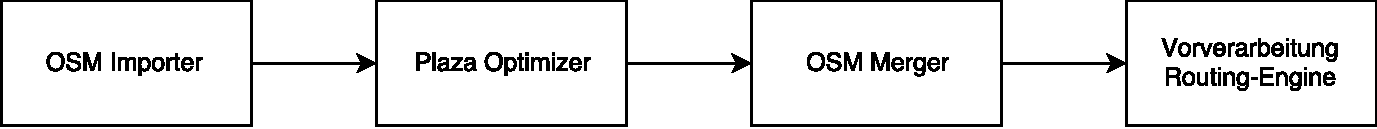
\includegraphics[width=1\linewidth]{projectdoc/img/dataflow_vorverarbeitung.pdf}
    \caption[Datenfluss Vorverarbeitung]{Datenfluss-Diagramm der Vorverarbeitung von \ac{OSM}-Daten bis zur Übergabe an die Routing-Engine; Grafik erstellt mit \emph{draw.io}}
    \label{fig:dataflow_vorverarbeitung}
\end{figure}


\begin{figure}[ht]
    \centering
    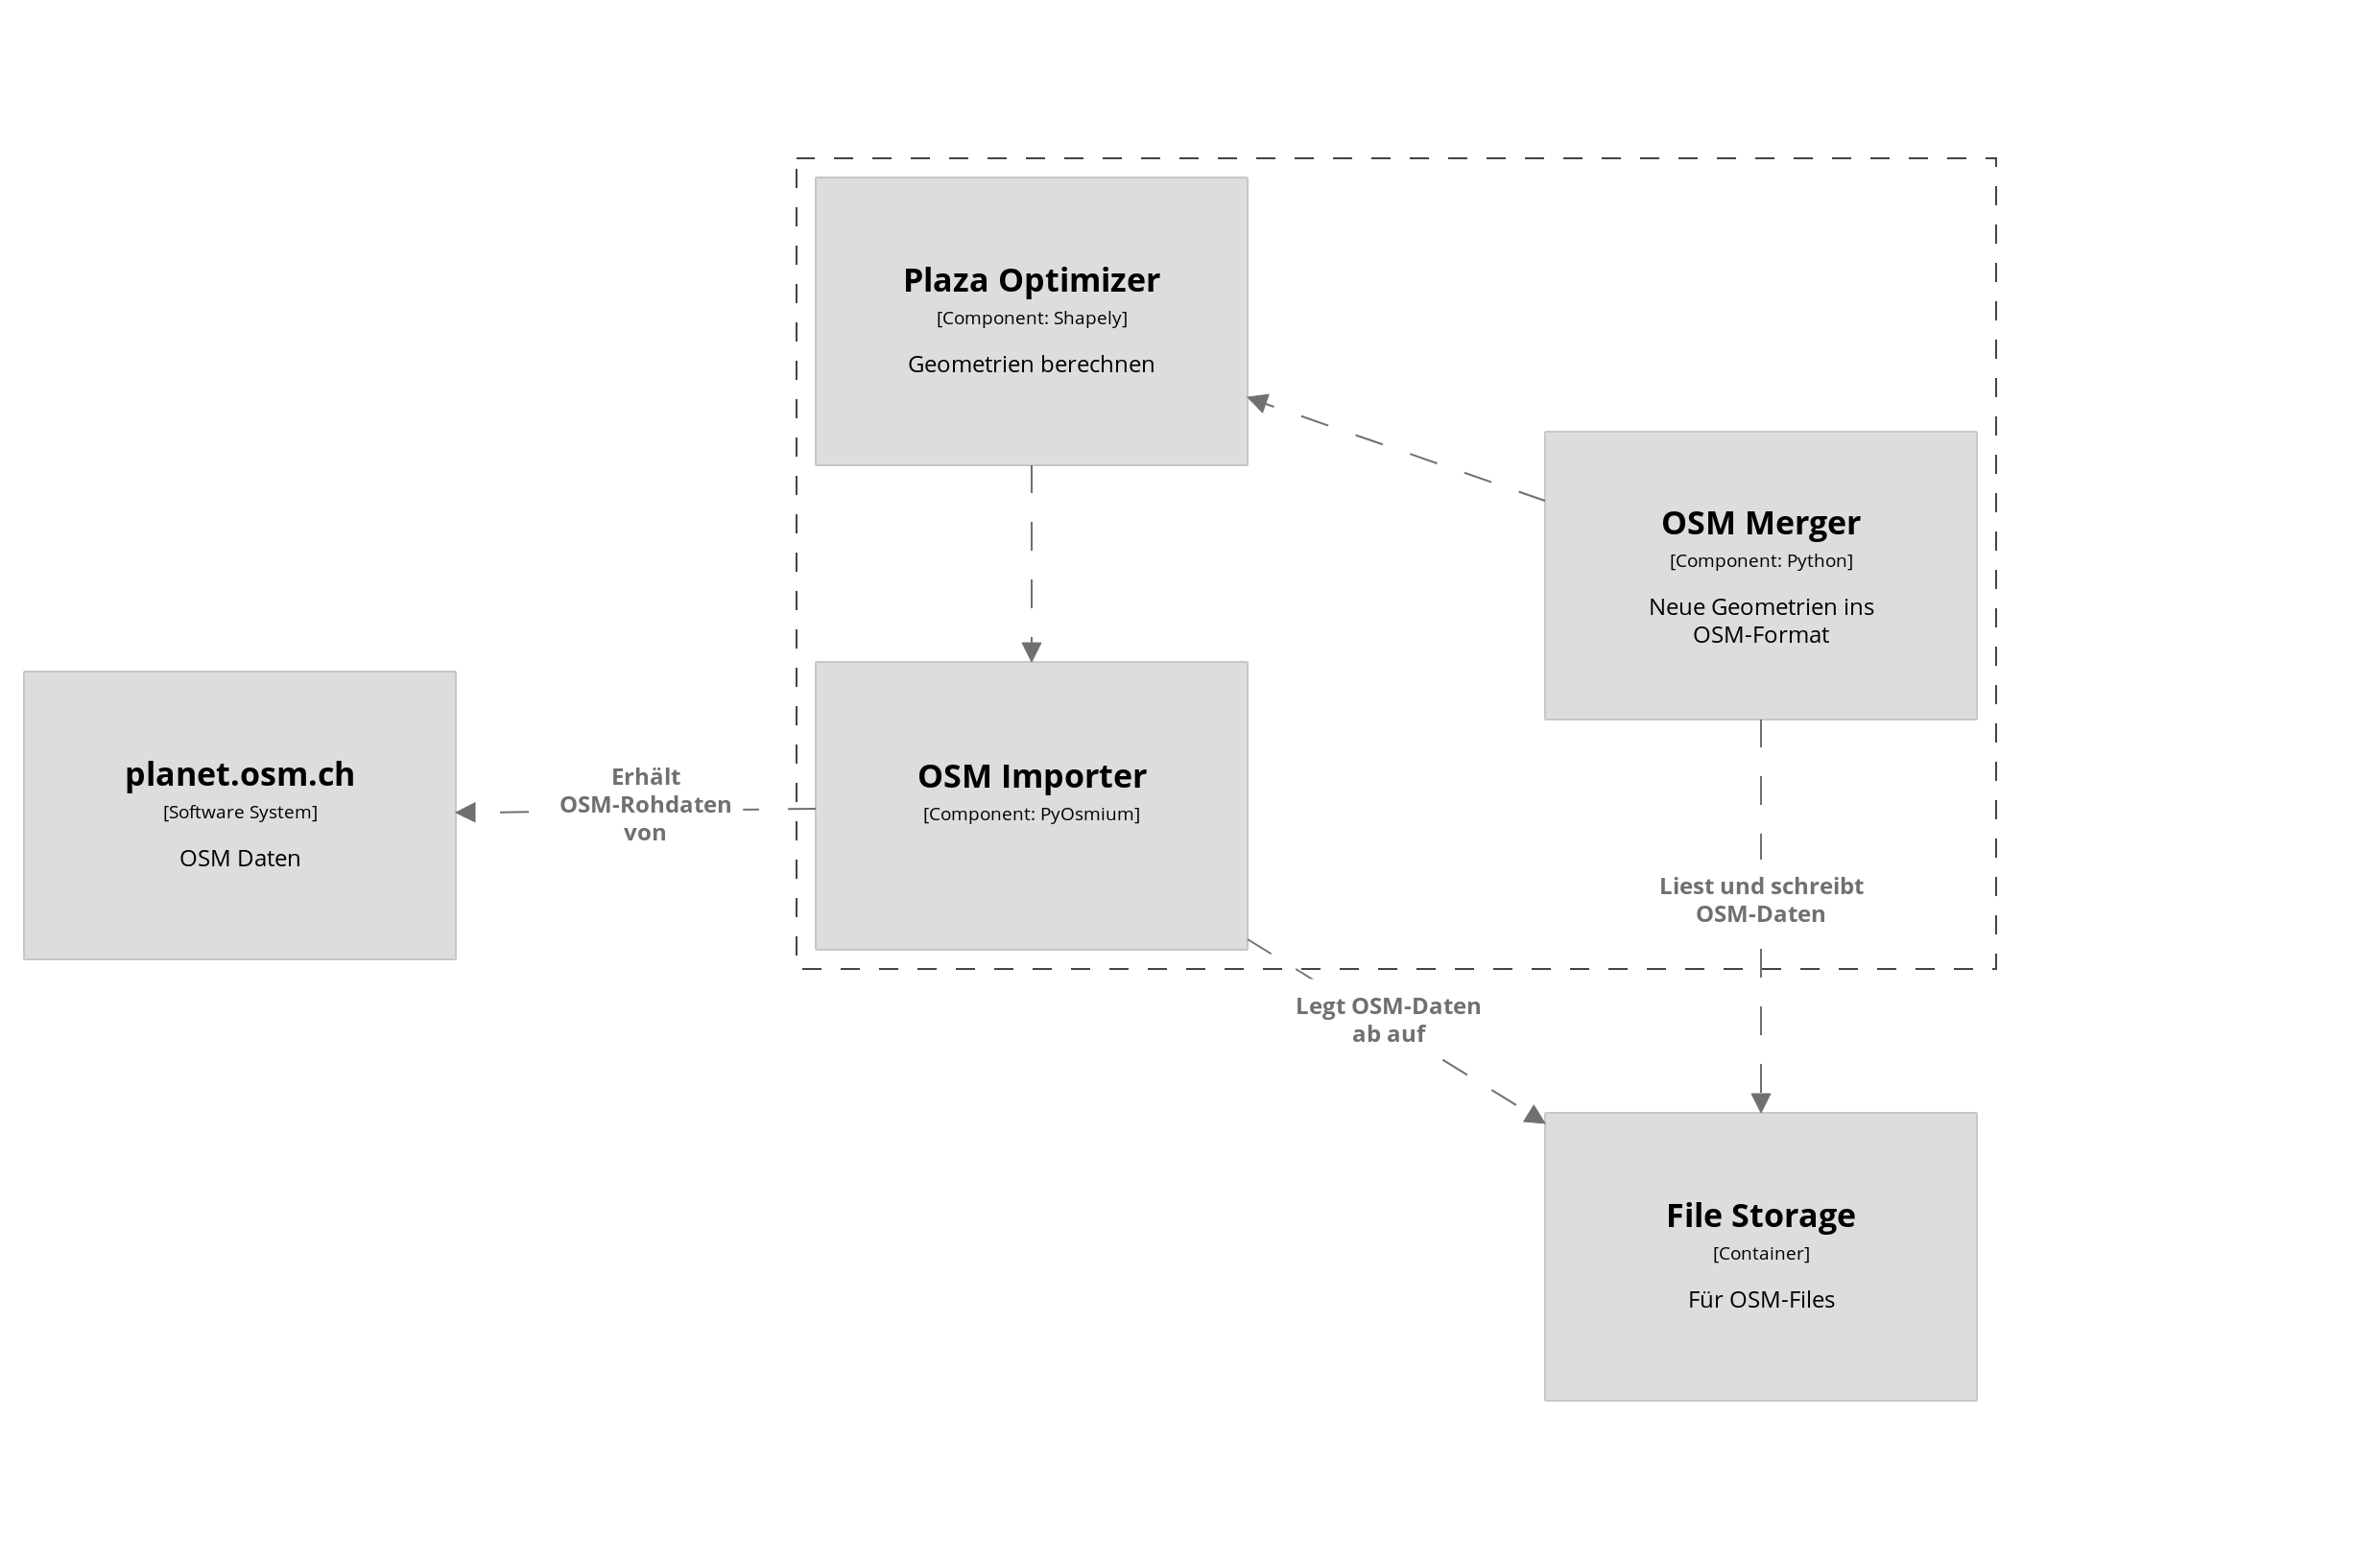
\includegraphics[width=1\linewidth]{projectdoc/img/component_diagram_plaza-vorverarbeitung.png}
    \caption[Komponentendiagramm Vorverarbeitung]{Komponentendiagramm der Plaza Vorverarbeitung (eingerahmt); Grafik erstellt mit \emph{Structurizr Express}\cite{structurizr}}
    \label{fig:component_diagram_vorverarbeitung}
\end{figure}


\paragraph{OSM Importer}\label{par:OSM Importer}~\\
Für unser optimiertes Routing wird in regelmässigen Abständen der neueste \ac{OSM}-Datensatz \cite{osm_data_switzerland} der Schweiz geladen. Die \acs{OSM}-Importer Komponente liest das komplette für uns relevante Kartenmaterial (z.B. die Schweiz) als \ac{PBF} ein und sucht dabei nach Flächen, die wir bearbeiten wollen.

Dazu werden \emph{Osmium} und die dazugehörigen Python-Bindings \emph{pyOsmium}\cite{pyosmium} verwendet. Osmium erkennt automatisch Flächen aus \ac{OSM} Multipolygone oder Relationen. Mit einem eigenen Handler können wir dabei gleich das Einlesen des Files auf die für uns interessanten Flächen beschränken.

\paragraph{Plaza Optimizer}\label{par:Plaza Optimizer}~\\
Die mit Osmium importierten \ac{OSM}-Daten sind noch reine \ac{OSM}-Objekte, auf denen keine Geometrie-Berechnungen angewendet werden können. Dazu wird die Python-Library \emph{Shapely}\cite{shapely} verwendet. Shapely kann mit Geometrien umgehen und Algorithmen von \ac{GEOS} wie \code{intersection} und \code{contains} darauf anwenden.

Um die mit Osmium importierten Objekte in Shapely zu verwenden, werden diese ins \ac{WKB} Format übersetzt und Shapely übergeben, wie in Listing \ref{shapely_import_code} gezeigt.

\begin{listing}[ht]
    \inputminted{python}{projectdoc/listing/shapely_import.py}
    \caption[Einlesen OSM Objekte in Shapely]{Übergabe von Osmium-Objekten zu Shapely für die Weiterverarbeitung}
    \label{shapely_import_code}
\end{listing}



\paragraph{OSM Merger}\label{par:OSM Merger}~\\
Der OSM Merger ist dafür verantwortlich, unsere erzeugten Geometrien (Fusswege) wieder in das \ac{OSM}-Kartenmaterial einzupflegen, um es anschliessend der Routing-Engine zur Verarbeitung zum Routing-Graphen zu übergeben.

Die durch unseren Algorithmus erzeugten Wege durch Flächen (in Shapely Datenstrukturen) sollen nun wieder zurück ins \ac{OSM}-Format geschrieben werden. Dazu wird wie beim \nameref{par:OSM Importer} Osmium verwendet, mit dem Geometrien in eine OSM-Datei geschrieben werden können

In einem weiteren Schritt müssen unsere optimierten Wege in das bestehende Strassennetz eingebunden werden, damit die Routing-Engine diese auch beachtet. Dazu werden die \glspl{Einstiegspunkt} der von uns erzeugten Fusswege in den bestehenden Strassen und Wegen referenziert, die an diesem Punkt auf die Fläche treffen. Somit werden sie topologisch direkt miteinander verbunden.

Als letzten Schritt führen wir die erzeugten Fusswege und die modifizierten Strassen wieder zusammen mit der "grossen" \ac{OSM}-Datei, die ganz am Anfang importiert wurde. Dazu wird das Commandline-Tool Osmosis \cite{osmosis} verwendet.

\subsubsection{Plaza Routing}
\label{architektur:Plaza Routing}
Der Plaza Routing Container (siehe Abbildung \ref{fig:container_diagram}) ist für das Koordinieren und Verarbeiten von Routing-Anfragen verantwortlich. Er bietet für das QGIS-Plugin eine API an. Mit Hilfe von verschiedenen Drittsystemen und der Routing-Engine (für Fussgänger-Routing) wird eine komplette Route mit Fahrplan erstellt und dem QGIS-Plugin oder anderen Konsumenten übergeben.

In diesem Abschnitt wird vertieft in die einzelne Bestandteile des Plaza Routing eingegangen. So sind nachfolgend die einzelnen Schichten und Konstrukte aufgeführt und beschrieben. Zur Übersicht findet man das Schichten-Diagramm in Abbildung \ref{fig:package_diagram_plaza_routing}. Die Verantwortlichkeiten der Drittsystemen wird in den jeweiligen Schichten angesprochen.

\begin{figure}[ht]
\centering
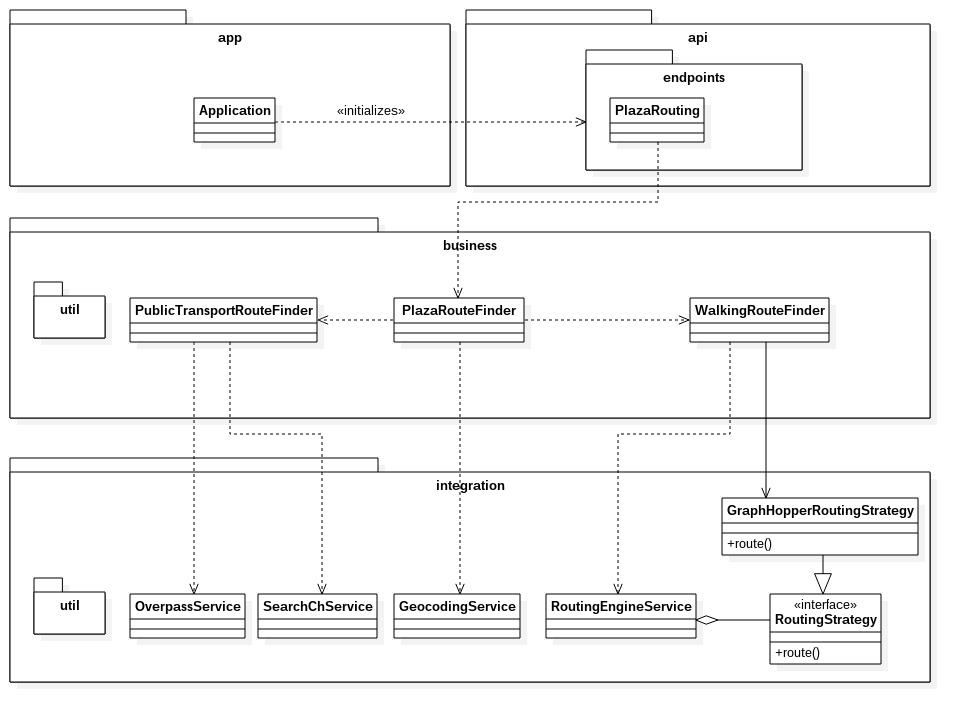
\includegraphics[width=1\linewidth]{projectdoc/img/package_diagram}
\caption[Schichten-Diagramm Plaza Routing]{Schichten-Diagramm Plaza Routing}
\label{fig:package_diagram_plaza_routing}
\end{figure}

\paragraph{app}\label{architektur:app-layer}~\\
Hierbei handelt es sich um den zentralen Einstiegspunkt in die Komponente \emph{PlazaRouting}. Die Komponenten wird in dieser Schicht konfiguriert und initialisiert.

\paragraph{api}\label{architektur:api-layer}~\\
In dieser Schicht wird eine \ac{REST}-\ac{API} für den gesamten externen Einstieg in das Plaza Routing exponiert. Diese \ac{API} wird primär vom \nameref{architektur:QGIS Plugin} verwendet. Eine Einschränkung bezüglich der Konsumenten gibt es nicht.

Die \ac{OAS} \cite{open-api-specificaiton} der \ac{API} ist unter \cite{plaza-routing-api-spez} verfügbar. SwaggerUI kann unter \cite{plaza-routing-api-swaggerui} eingesehen werden. Die {API}-Spezifikation wird in einem Git-Repository gehalten. Änderungen werden somit automatisch auf der Github-Page \cite{plaza-routing-api-spez} publiziert. Dies hat die Vorteile, dass es keine Abweichung zwischen Spezifikation und Dokumentation geben kann, mit Swagger \cite{swagger} die Schnittstelle bereits ideal beschrieben ist und die Haltung in einem öffentlichen Repository eine Diskussions-Plattform für Konsumenten bietet.

\paragraph{business}\label{architektur:business-layer}~\\
In der Business-Schicht ist die Business-Logik der \ac{API}-Abfragen vorhanden. Das PlazaRouting wird logisch in zwei Bereiche \emph{PublicTransportConnectionFinder} und \emph{WalkingRouteFinder} aufgeteilt. Die Koordination übernimmt dabei \emph{PlazaRouteFinder}. So wird das Design-Prinzip \emph{Separation of Concern} ideal umgesetzt, da \emph{PublicTransportConnectionFinder} nur mit Services kommuniziert, welche für das ÖV-Routing notwendig sind und \emph{WalkingRouteFinder} die Kommunikation mit der Routing-Engine übernimmt.

\paragraph{integration}\label{architektur:integration-layer}~\\
In den nachfolgenden Abschnitten sind die Integration-Services und ihre Notwendigkeit beschrieben. In dieser Architektur werden Komponenten, welche mit Drittsystemen oder -komponenten kommunizieren als \emph{Services} bezeichnet und der Integration-Schicht angegliedert.

\subparagraph{Search.ch Service}\label{architektur:Search.ch Service}~\\
Der \emph{SearchChService} kommuniziert mit der Fahrplan-\ac{API} von search.ch \cite{search_ch_route_api} und bezieht die Fahrplan-Daten für eine bestimmte Ausgangsstation und Destination.

\subparagraph{Overpass Service}\label{architektur:Overpass Service}~\\
Der \emph{OverpassService} übernimmt mithilfe der \ac{QL} die Kommunikation mit Overpass \cite{wiki:overpass}. Der Hauptfokus liegt auf dem Extrahieren von ÖV-Stationen in einem gegebenen Umkreis und geografischen Position von ÖV-Stationen basierend auf Daten, welche aus dem \nameref{architektur:Search.ch Service} gewonnen werden.

\subparagraph{Geocoding Service}\label{architektur:Geocoding Service}~\\
Der \emph{GeocodingService} liefert für eine Adresse eine Koordinate.

\subparagraph{Routing-Engine Service}\label{architektur:Routing-Engine Service}~\\
Der \emph{RoutingEngineService} ist für das Fussgänger-Routing zuständig und kommuniziert mit einer Routing-Engine. Die Architektur ist mit dem Strategy-Pattern \cite{gof_patterns} so gewählt, dass die Routing-Engine einfach ausgetauscht werden kann.

\subsection{QGIS Plugin}
\label{architektur:QGIS Plugin}

Das QGIS-Plugin ist unabhängig vom System PlazaRoute und läuft auf dem Client des Benutzers. Die Kommunikation mit dem Container Plaza Routing erfolgt über einen REST-Service. Das Plugin ist reiner Konsument und zeigt auf, welchen Mehrwert PlazaRoute bieten kann. In Abbildung \ref{fig:class_diagram_plaza_route_qgis_plugin} ist das Klassen-Diagramm zu sehen. Herausheben kann man, dass das Plugin in fünf Komponente zerlegt wird. \emph{PlazaRouteRoutingService} kommuniziert mit dem REST-Service (siehe Abschnitt \nameref{architektur:api-layer}). \emph{PlazaRouteMapTool} übernimmt die Interaktion mit der Karte und führt das Zeichnen der Route mit \emph{PlazaRouteRouteDrawer} durch. \emph{PlazaRouteRoutingGenerator} generiert ein Routing für die zurückgelieferte Route. Die zentrale Steuerung übernimmt das Dockwidget.

\begin{figure}[th]
    \centering
    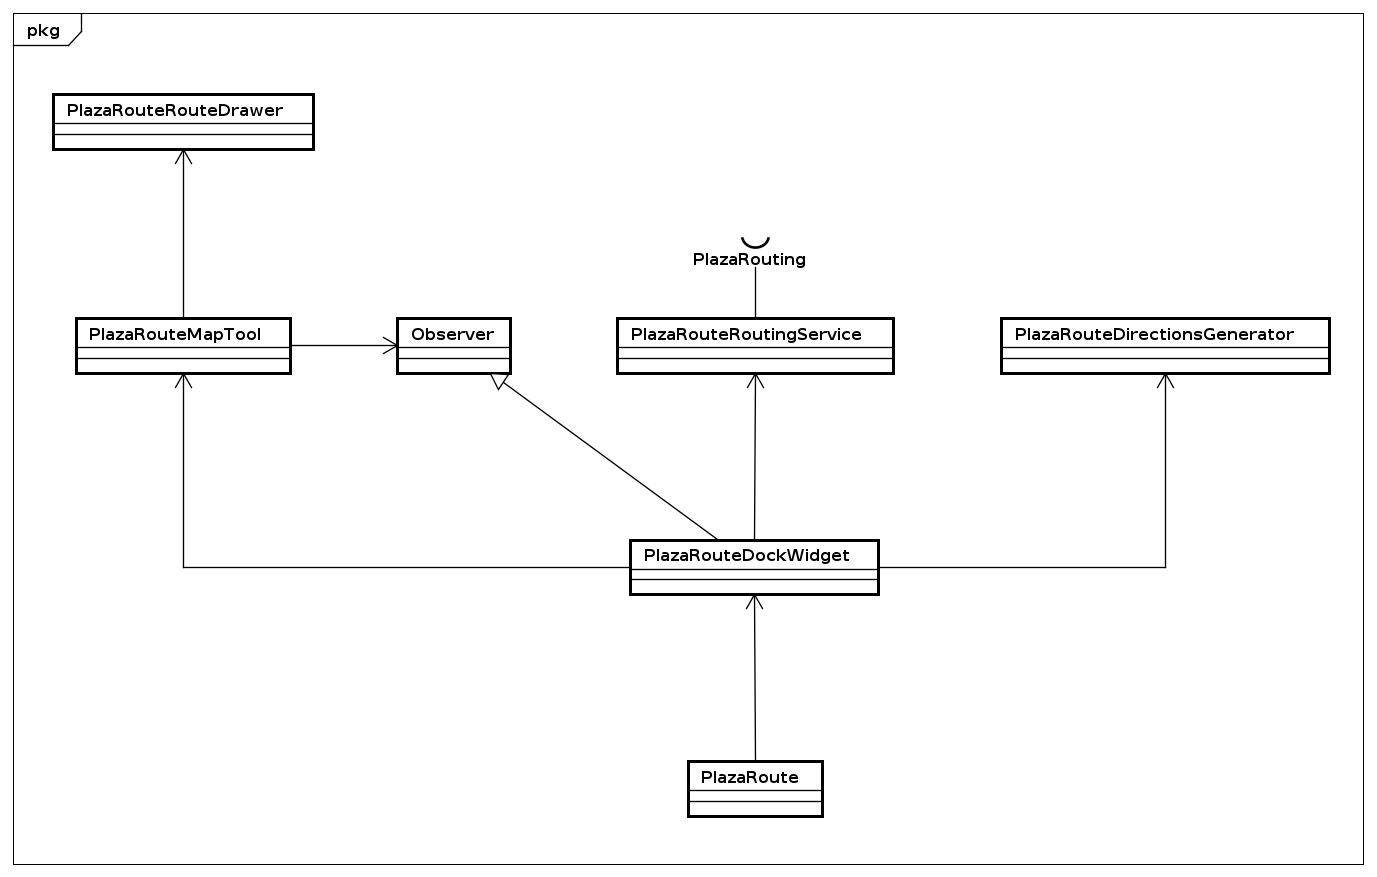
\includegraphics[width=1.0\linewidth]{projectdoc/img/class_diagram_plaza_route_qgis_plugin}
    \caption[Klassen-Diagramm Plaza Route QGIS Plugin]{Klassen-Diagramm Plaza Route QGIS Plugin}
    \label{fig:class_diagram_plaza_route_qgis_plugin}
\end{figure}

